\documentclass{beamer}

% Prepare for svenska tecken
\usepackage[T1]{fontenc}
\usepackage[utf8]{inputenc}
\usepackage[swedish]{babel}
%\usepackage[]{geometry}
\addto\captionsswedish{\renewcommand{\figurename}{Bild}}
\usepackage{amsmath}
\usepackage{fancyhdr}
\usepackage{wrapfig}
\usepackage{caption}
\usepackage{framed}
\usepackage[fulladjust]{marginnote}
\usepackage{color}
\newcommand{\hilight}[1]{\colorbox{yellow}{#1}}
\usepackage{hyperref}
\hypersetup{
    colorlinks,
    citecolor=black,
    filecolor=black,
    linkcolor=black,
    urlcolor=black
}
\usepackage{stmaryrd} % För symbolen \boxbox, kräver paketet texlive-math-extra

% % % % % % % % % % % 
% Detta är nya environments för review. De bör vara relativt självförklarande hur de används.
% I princip sätter man bara den del av texten som har en viss status mellan\begin{rev-granskat} och \end{rev-granskat} tex.
% Undvik att nästla dem för det är ingen idé det fungerar inte.
% De är testade med ett antal andra environemnt som tabular mm men kolla att det fungerar med de environments du använder.
% % % % % % % % % % % % % % % % % % % % % % % % % % % % % % % % % % % % % % % % % % % % % % % % % % % % % % % % % % % % % % % 
%\usepackage[svgnames,rgb]{xcolor}
%\usepackage{pdfcomment}
%\newenvironment{rev-ogranskat}{\begin{pdfsidelinecomment}[color=black,linewidth=3px,caption=inline]{Ogranskat}}{\end{pdfsidelinecomment}}
%\newenvironment{rev-omarbetas}{\begin{pdfsidelinecomment}[color=red,linewidth=3px,caption=inline]{Omarbetas}}{\end{pdfsidelinecomment}}
%\newenvironment{rev-raderas}{\begin{pdfsidelinecomment}[color=red,linewidth=3px,caption=inline]{Raderas}}{\end{pdfsidelinecomment}}
%\newenvironment{rev-redo}{\begin{pdfsidelinecomment}[color=yellow,linewidth=3px,caption=inline]{Redo att granska}}{\end{pdfsidelinecomment}}
%\newenvironment{rev-granskat}[1][]%
%{\begin{pdfsidelinecomment}[color=green,linewidth=3px,caption=inline]%
%{Granskat #1}}%
%{\end{pdfsidelinecomment}}
%\newenvironment{rev-nytt}[1][]%
%{\begin{pdfsidelinecomment}[color=brown,linewidth=3px,caption=inline]%
%{Nytt #1}}%
%{\end{pdfsidelinecomment}}
%\newenvironment{rev-releasat}{\begin{pdfsidelinecomment}[color=blue,linewidth=3px,caption=inline]{Klart}}{\end{pdfsidelinecomment}}

%\clubpenalty=9990
%\widowpenalty=9999
%\brokenpenalty=4999

\usepackage[europeanvoltages,europeancurrents,europeanresistors,cuteinductors,smartlabels]{circuitikz}
\usepackage[framemethod=TikZ]{mdframed}

\mdfdefinestyle{FactBox}{%
    linecolor=blue,
    outerlinewidth=2pt,
    roundcorner=20pt,
    innertopmargin=\baselineskip,
    innerbottommargin=\baselineskip,
    innerrightmargin=20pt,
    innerleftmargin=20pt,
    backgroundcolor=gray!50!white}
\newcommand{\infobox}[1]{
\begin{wrapfigure}{r}{0.5\textwidth}
  \begin{mdframed}[style=FactBox]
#1
  \end{mdframed}
\end{wrapfigure}
}

% Make some unicode characters usable
\DeclareUnicodeCharacter{00B0}{\ensuremath{^\circ}} % unicode 00B0 ° degree sign
\DeclareUnicodeCharacter{00B5}{\ensuremath{\mu}} % unicode 00B5 µ micro sign
\DeclareUnicodeCharacter{03C0}{\ensuremath{\pi}} % unicode 3C0 π greek small letter pi
\DeclareUnicodeCharacter{03A9}{\ensuremath{\Omega}} % unicode 3A9 Ω greek capital letter omega
\DeclareUnicodeCharacter{2206}{\ensuremath{\Delta}} % unicode 2206 ∆ increment


% Prepare for tables
\usepackage{multirow}
\usepackage{longtable}

% Prepare for lists
%\usepackage{enumitem}

% Prepare for graphics
\usepackage{xspace,graphicx}

\raggedbottom


%% Frontpage bacground
\usepackage{eso-pic}
\newcommand\BackgroundPic{%
\put(0,0){%
\parbox[b][\paperheight]{\paperwidth}{%
\vfill
\centering
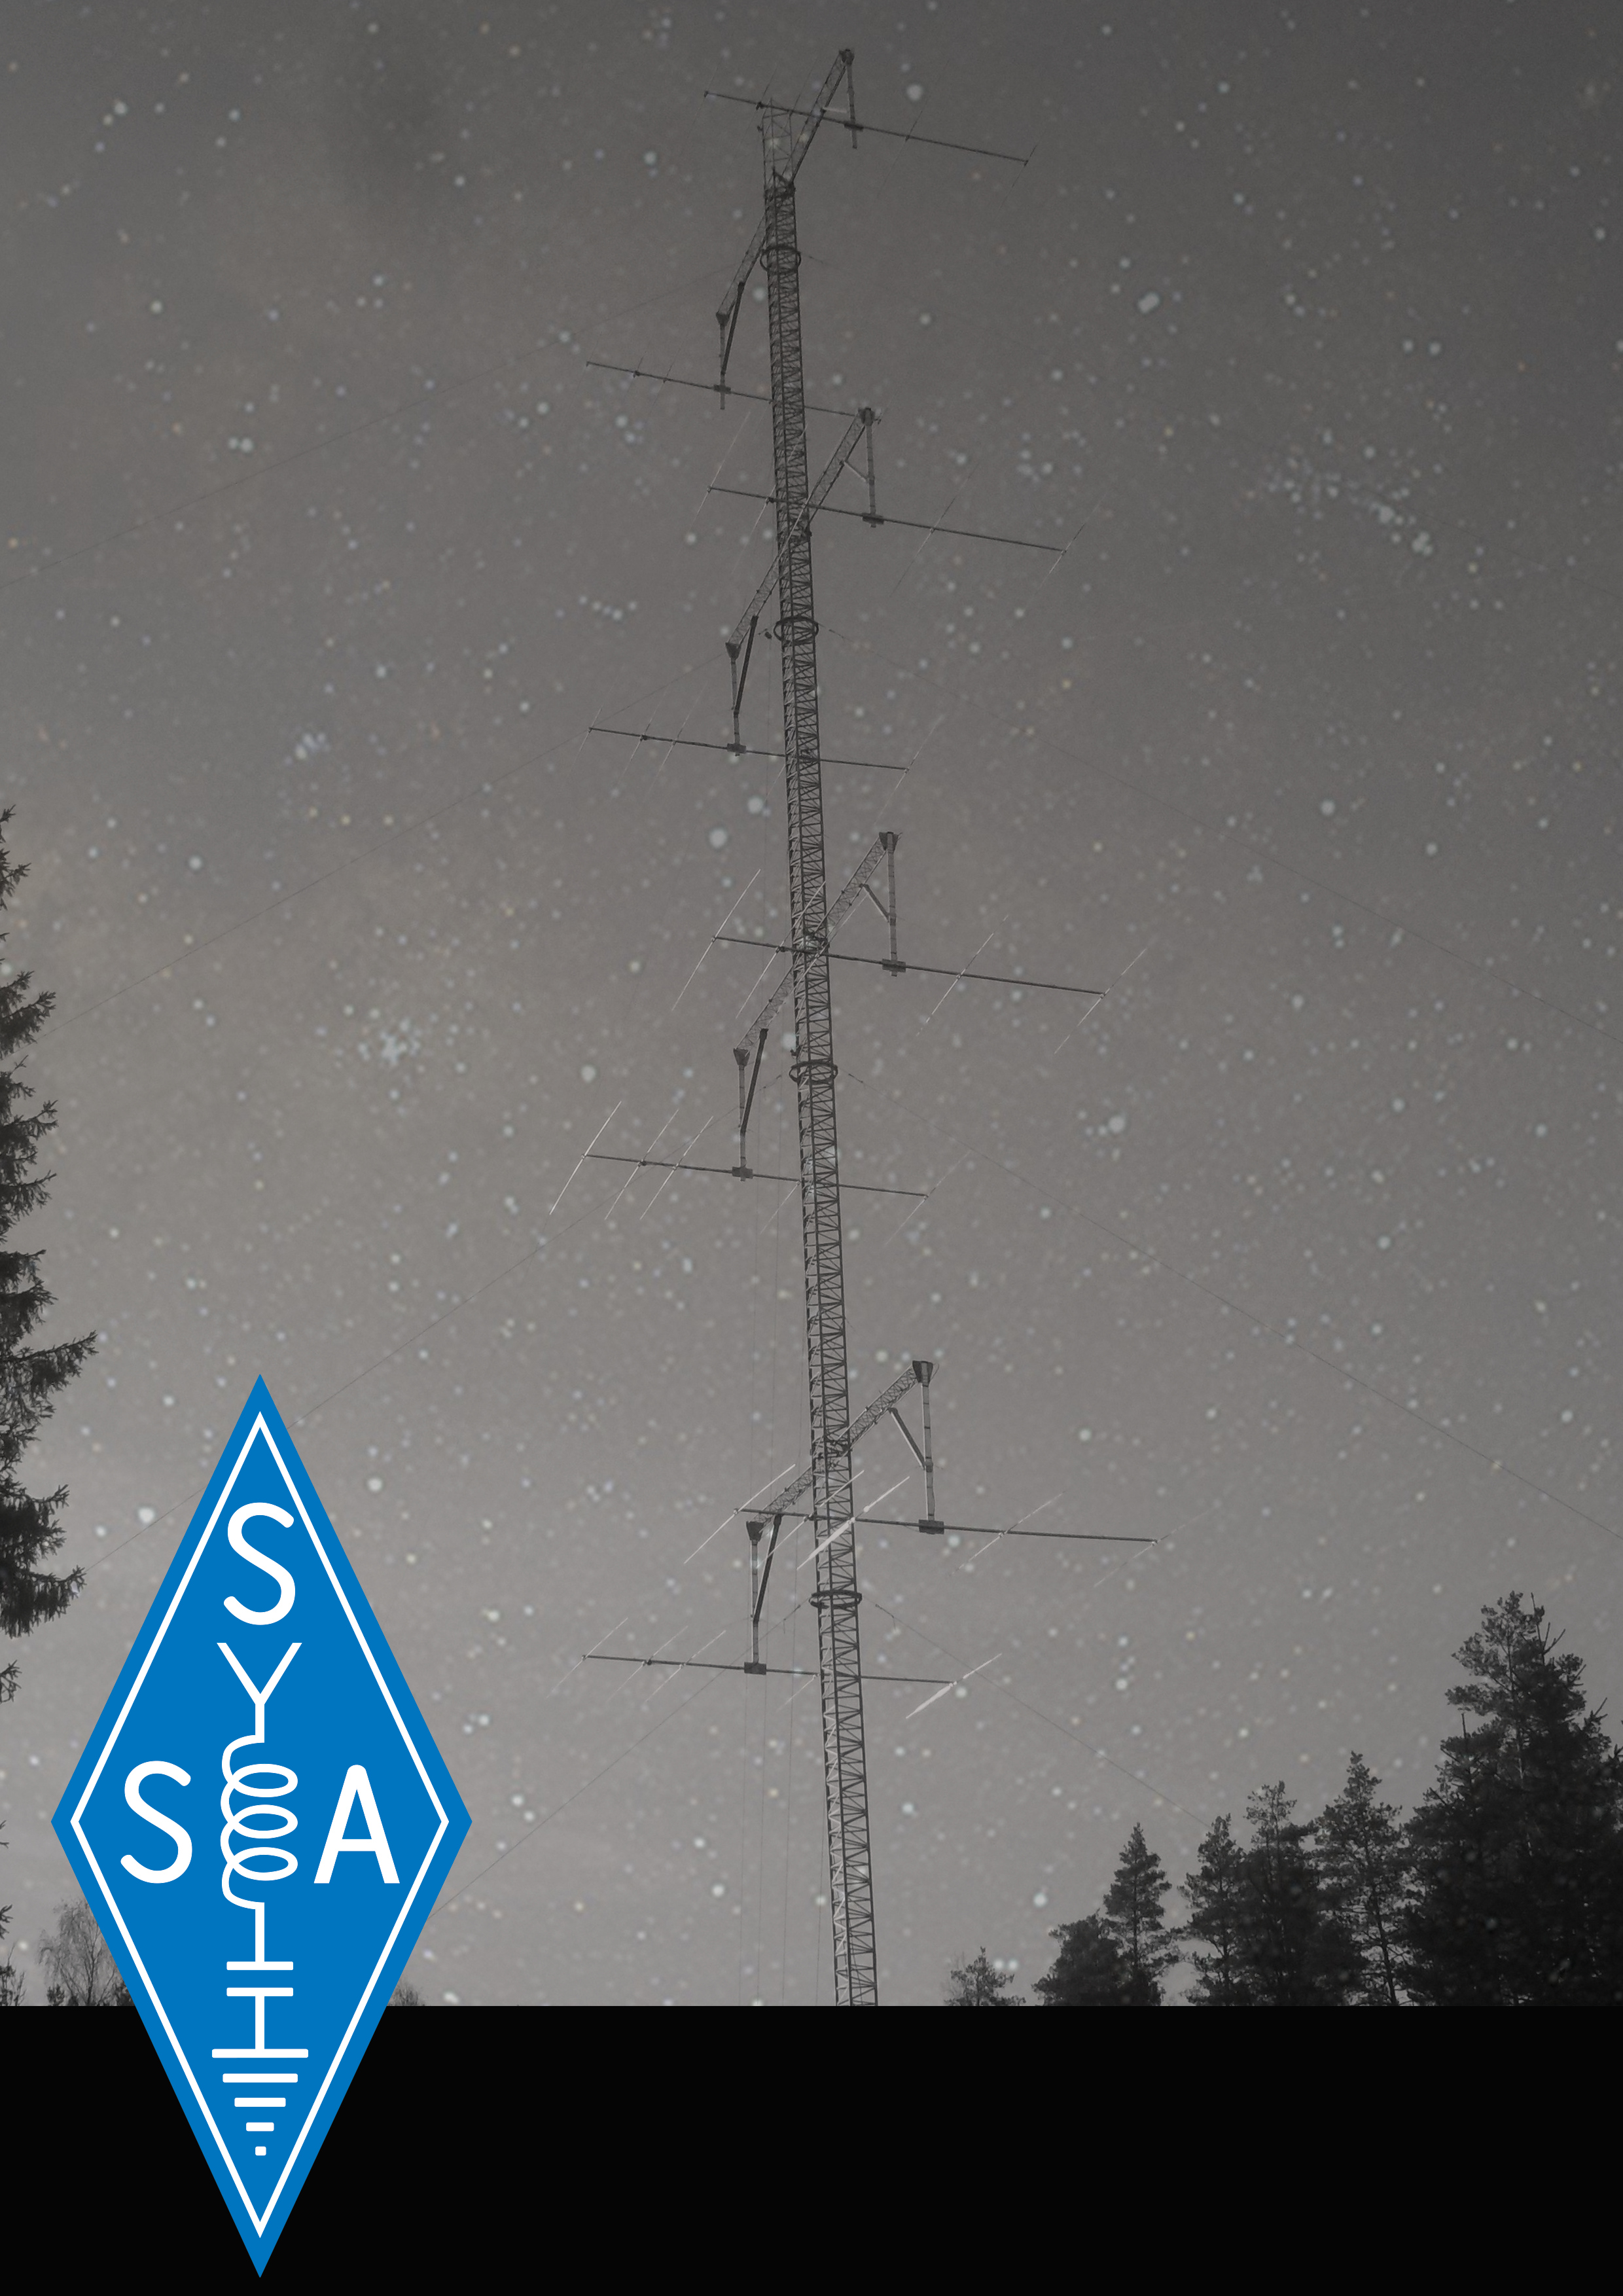
\includegraphics[width=\paperwidth,height=\paperheight,%
keepaspectratio]{images/koncept-front.jpg}%
\vfill
}}}


\newcommand\BackgroundPicLast{%
\put(0,0){%
\parbox[b][\paperheight]{\paperwidth}{%
\vfill
\centering
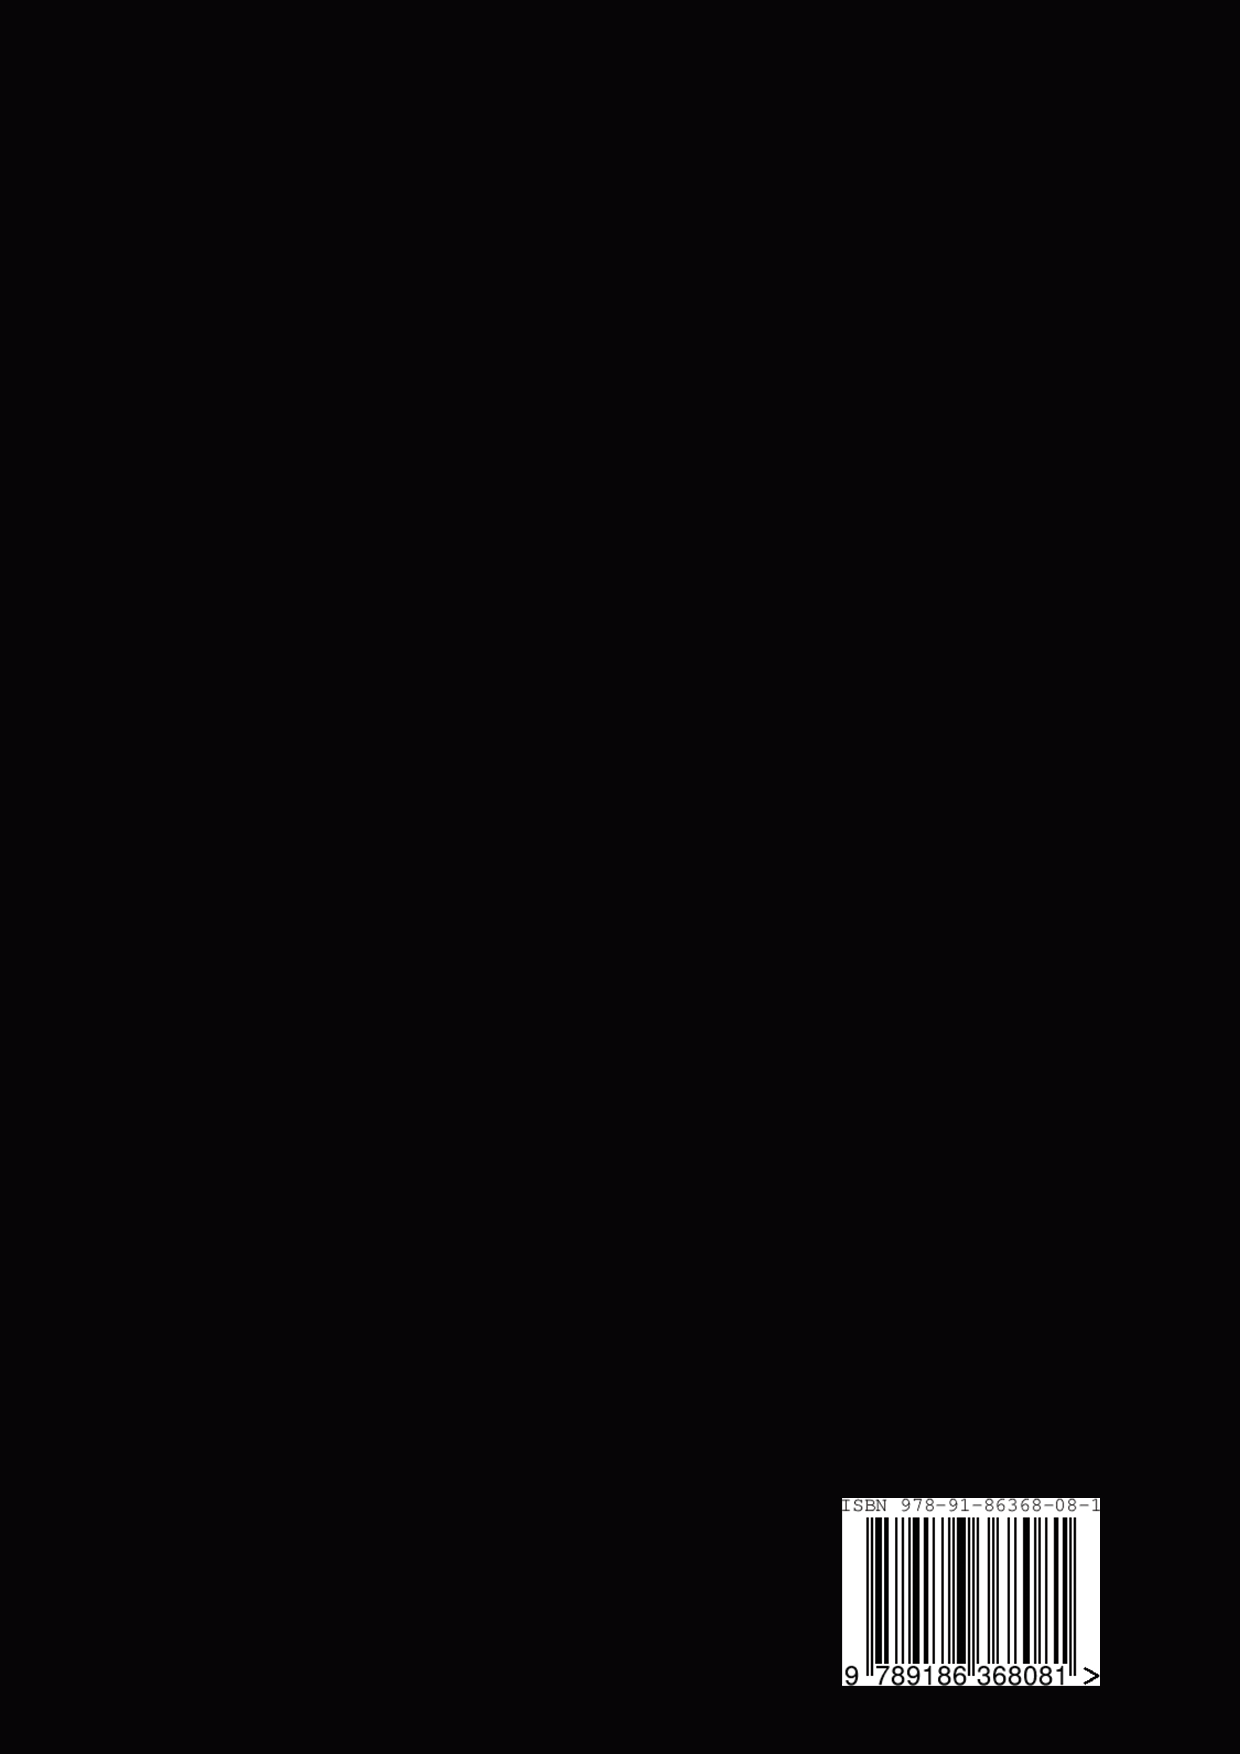
\includegraphics[width=\paperwidth,height=\paperheight,%
keepaspectratio]{images/koncept-back.pdf}%
\vfill
}}}

\usepackage[swedish]{babel}

\mode<presentation>
{
\usetheme{Madrid}
\usecolortheme{default}
\usefonttheme{serif}
\setbeamertemplate{navigation symbols}{}
\setbeamertemplate{caption}[numbered]
}
\usepackage{tikz}
\usepackage{amsmath,amsfonts,amssymb,bm,mathrsfs}
\usetikzlibrary{shapes,arrows}

\title{Halvledare, förstärkare, oscillatorer}
\author{Magnus Danielson SA0MAD}

\begin{document}

\begin{frame}
\titlepage

\includegraphics[height=0.3\textheight]{images/ssalogo}
\end{frame}

\begin{frame}{Outline}
\tableofcontents
\end{frame}

\section{Halvledare}

\begin{frame}{PN-övergången}

\begin{figure}[h]
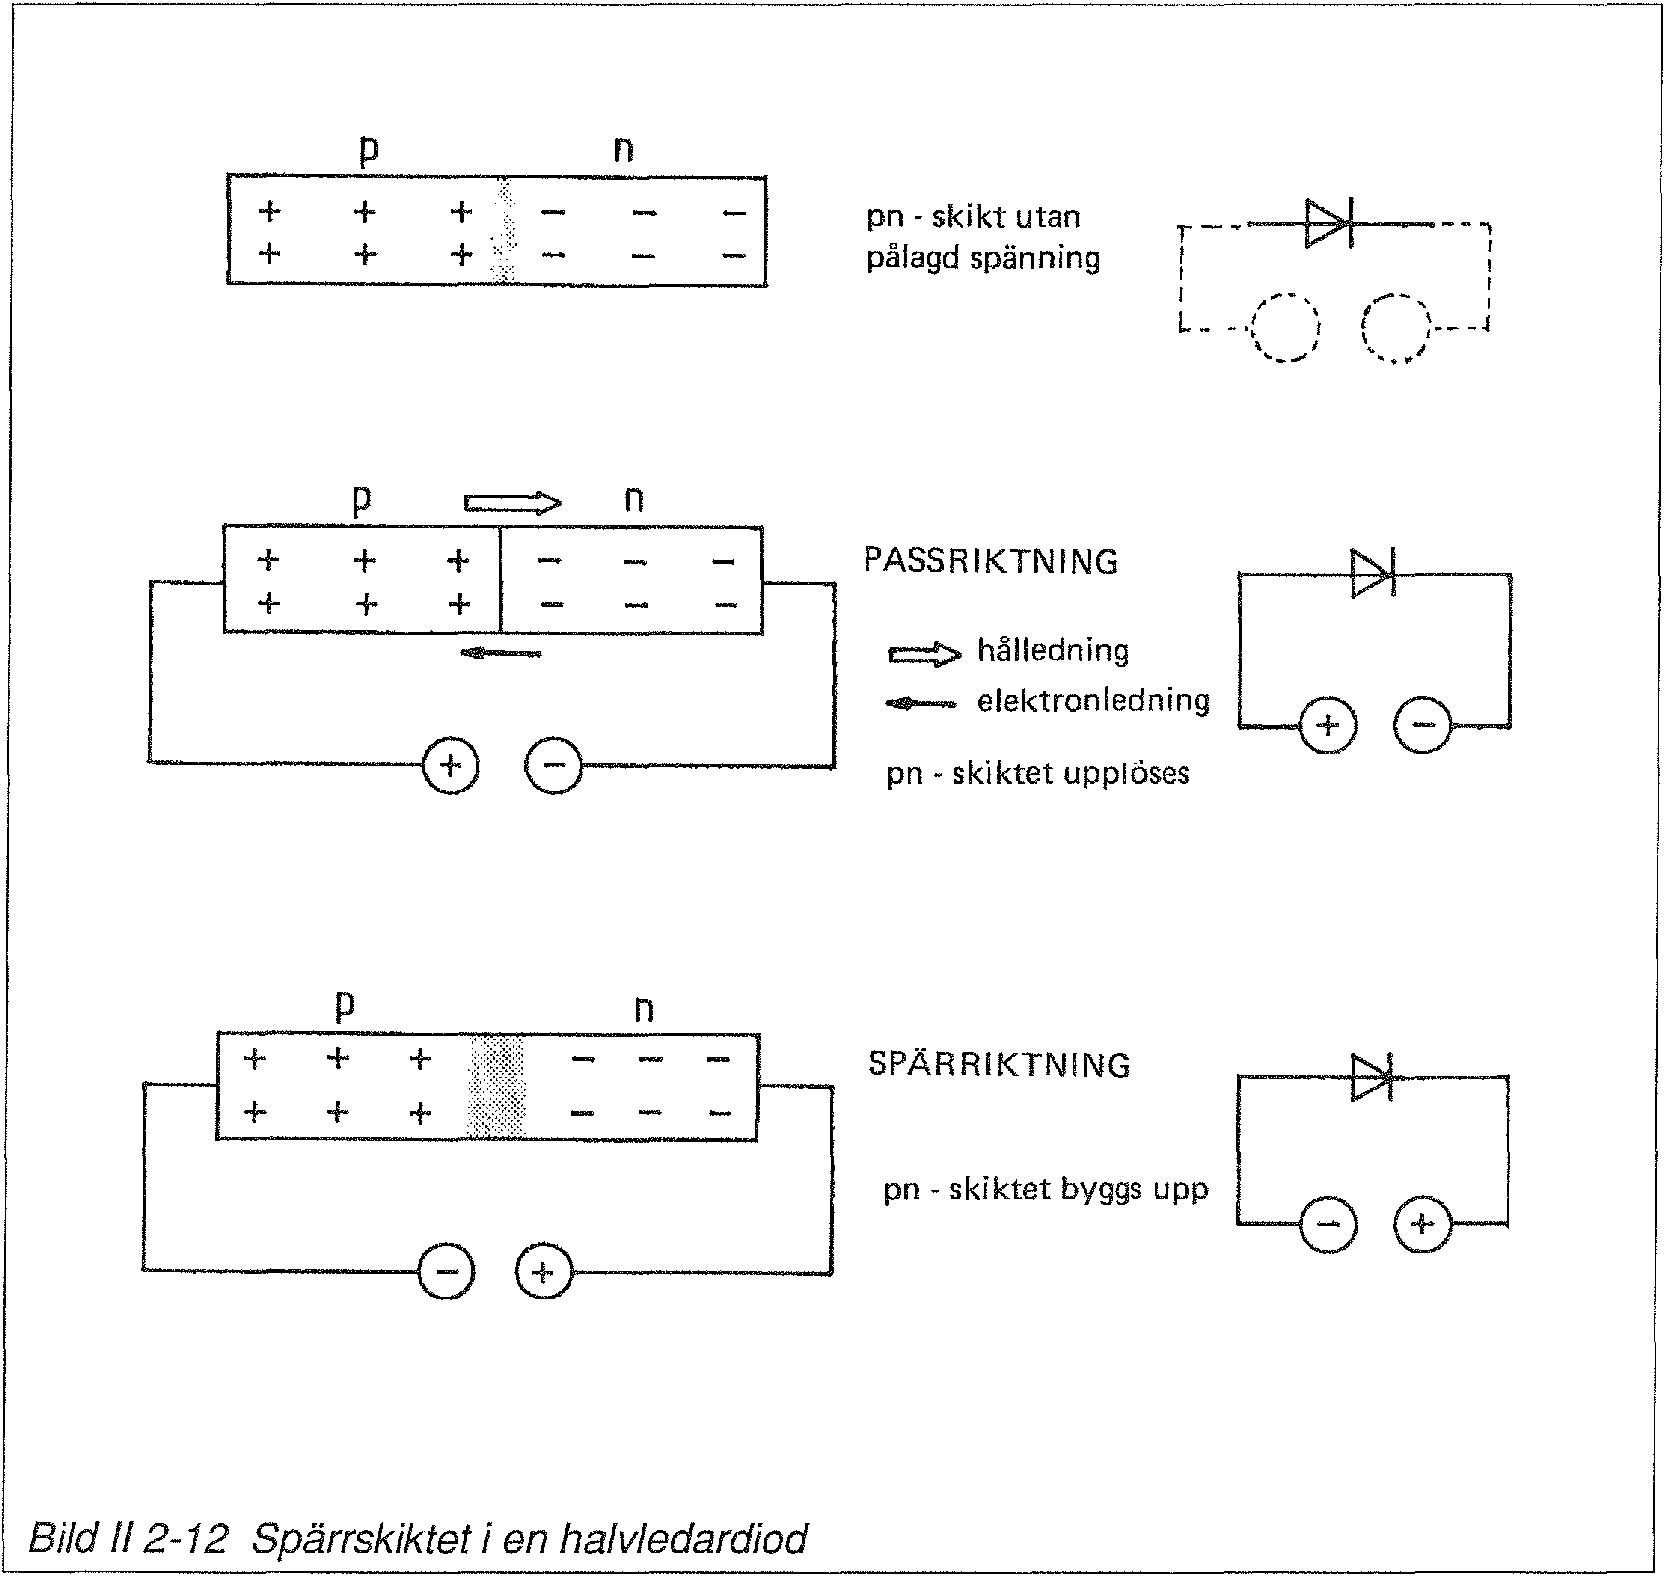
\includegraphics[width=0.6\textwidth]{images/bild_2_2-12}
%\caption{Alstring av en sinusformad signal}
\label{fig:BildII1-16}
\end{figure}
\end{frame}

\begin{frame}{Halvledardioden}

\begin{figure}[h]
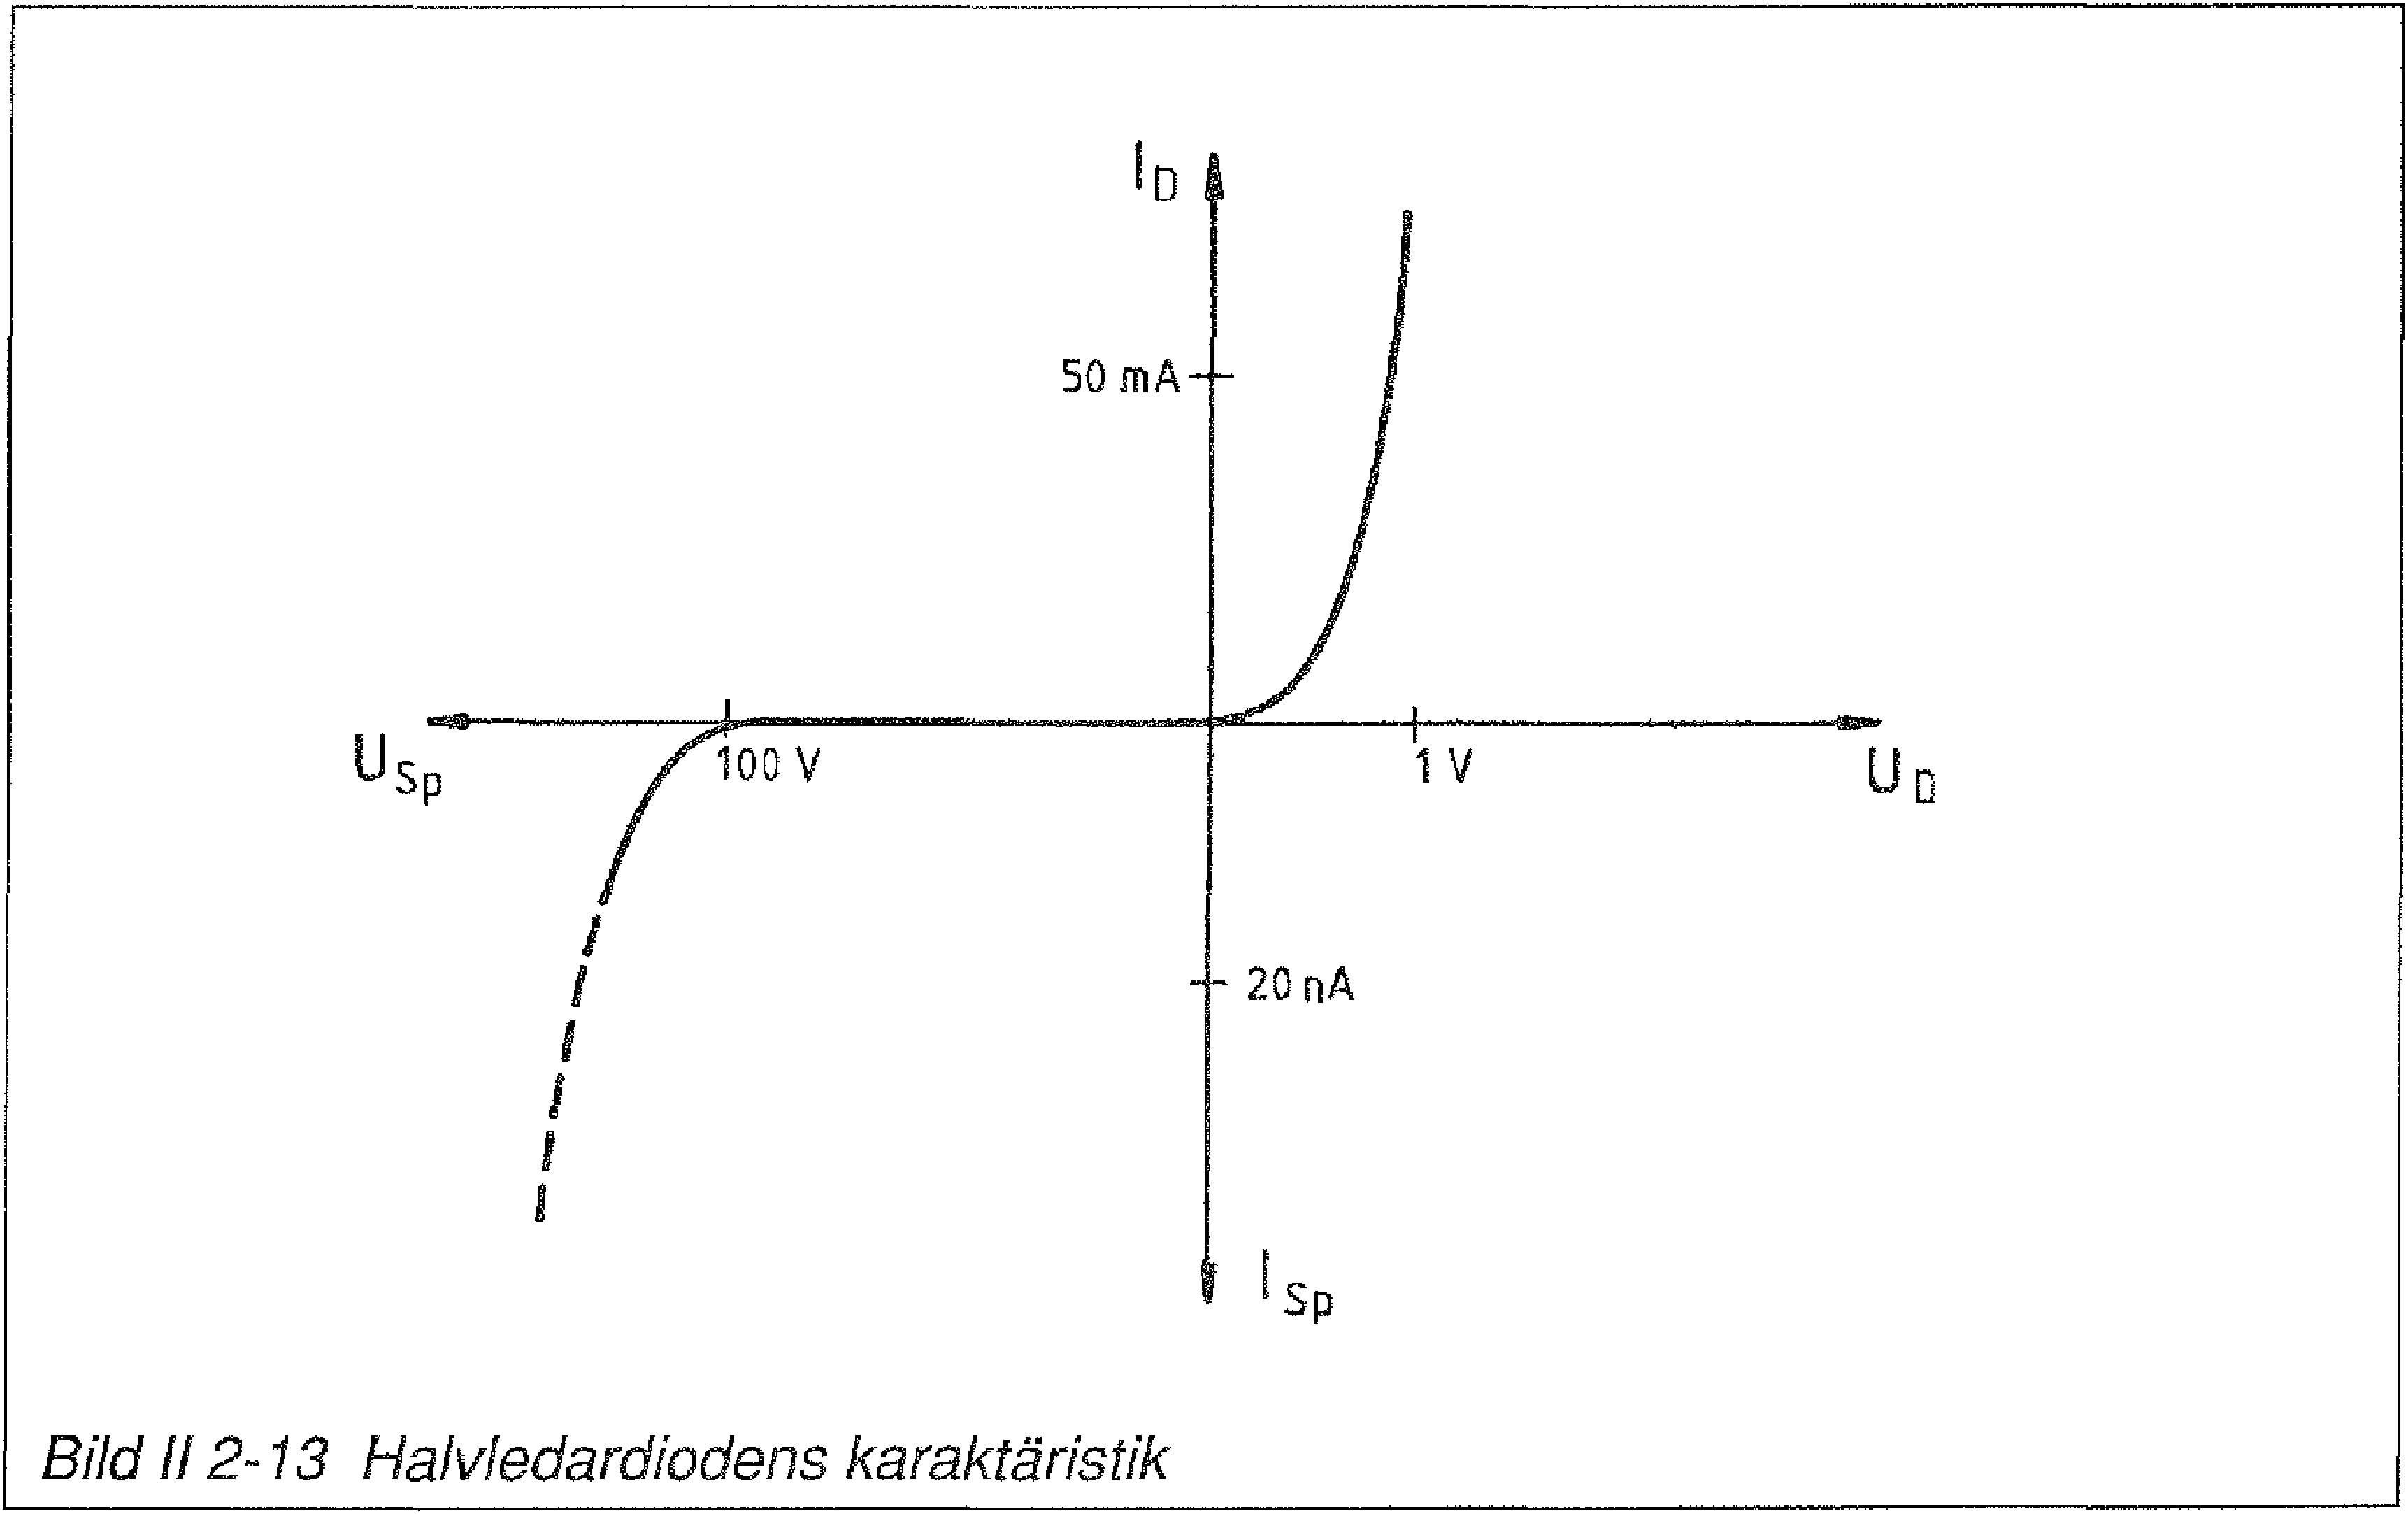
\includegraphics[width=0.6\textwidth]{images/bild_2_2-13}
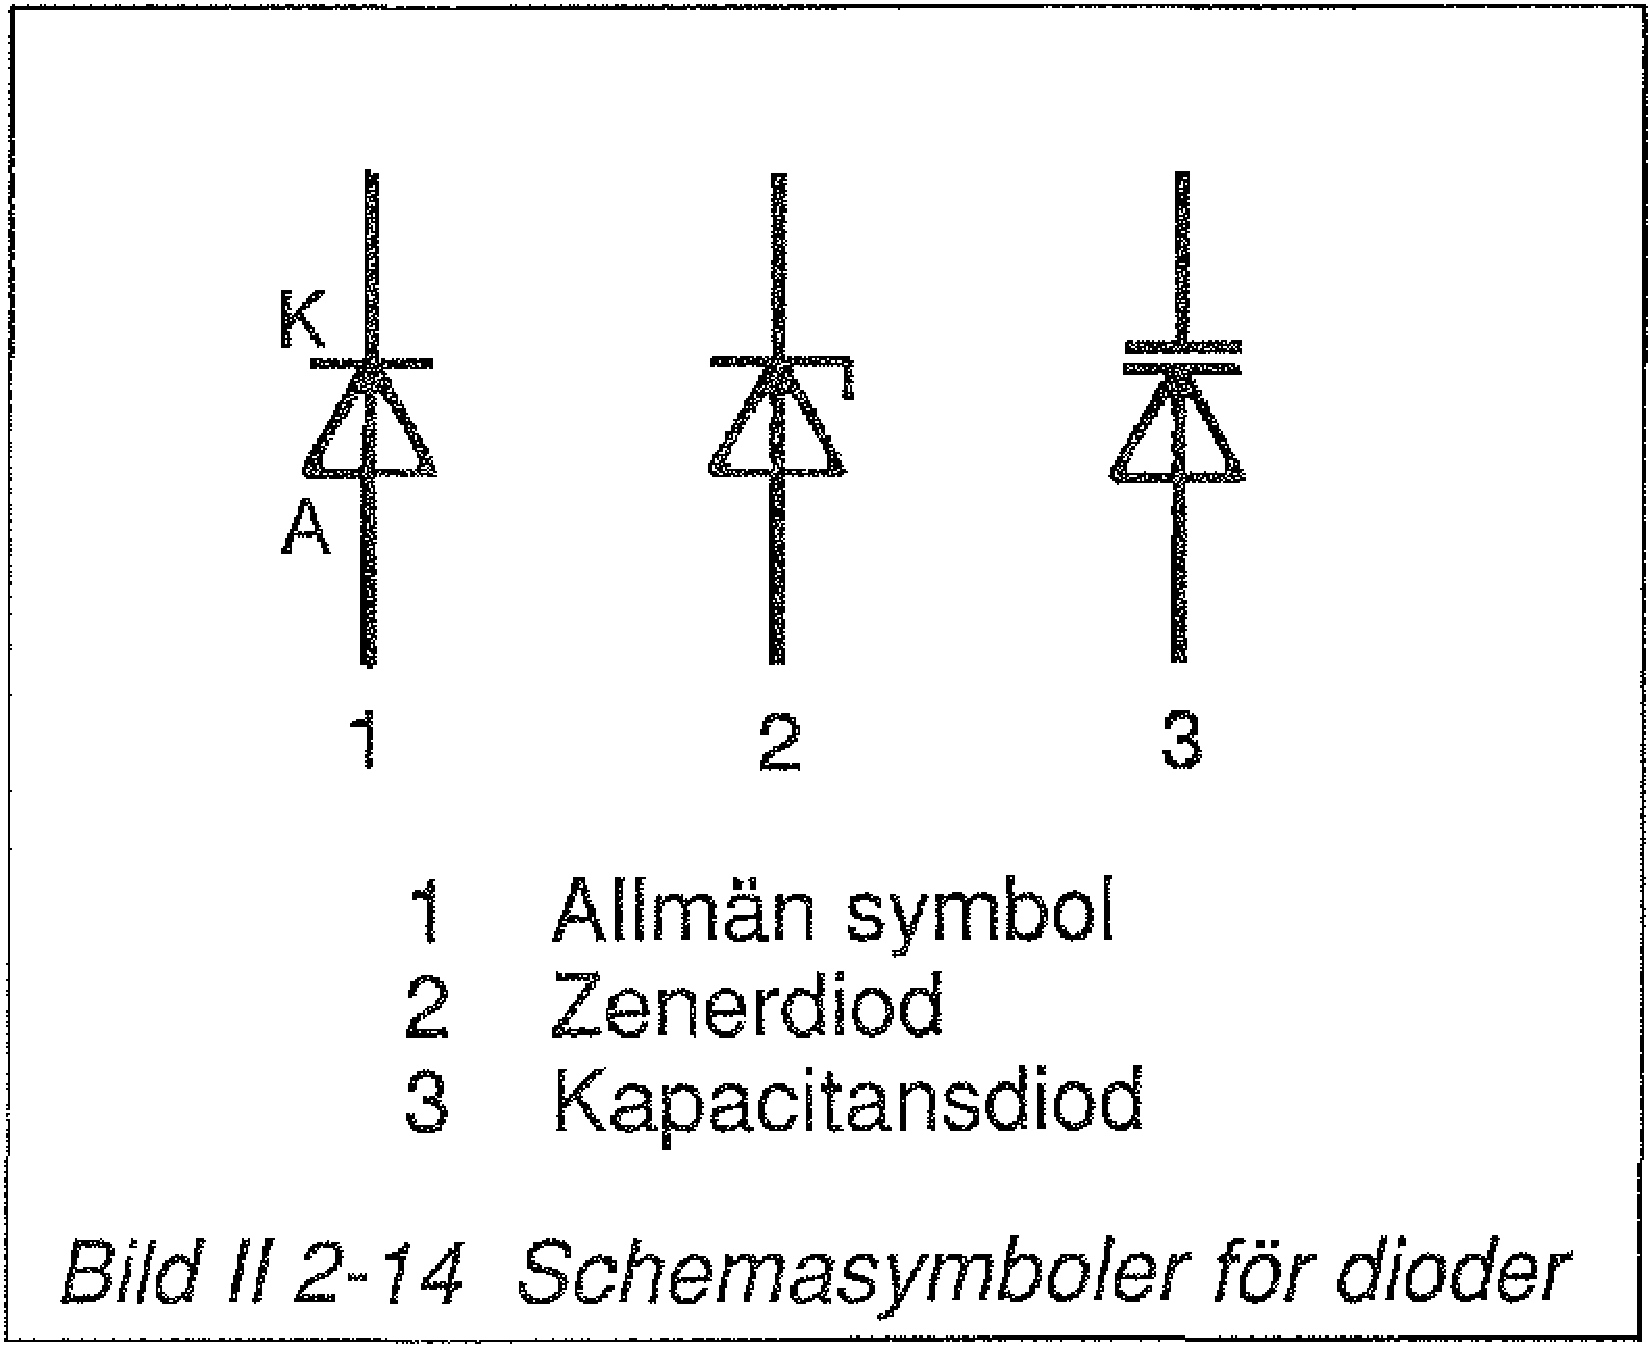
\includegraphics[width=0.4\textwidth]{images/bild_2_2-14}
%\caption{Alstring av en sinusformad signal}
\label{fig:BildII1-16}
\end{figure}

\begin{itemize}
  \item Olinjärt förhållande mellan spänning och ström
  \item Leder ström huvudsakligen åt enbart ett håll
  \item I backriktningen aggerar den kondensator vars kapacitans beror på pålagd spänning
  \end{itemize}
\end{frame}

\section{Kraftaggregat}

\begin{frame}{Kraftaggregat -- likriktning}

\begin{figure}[h]
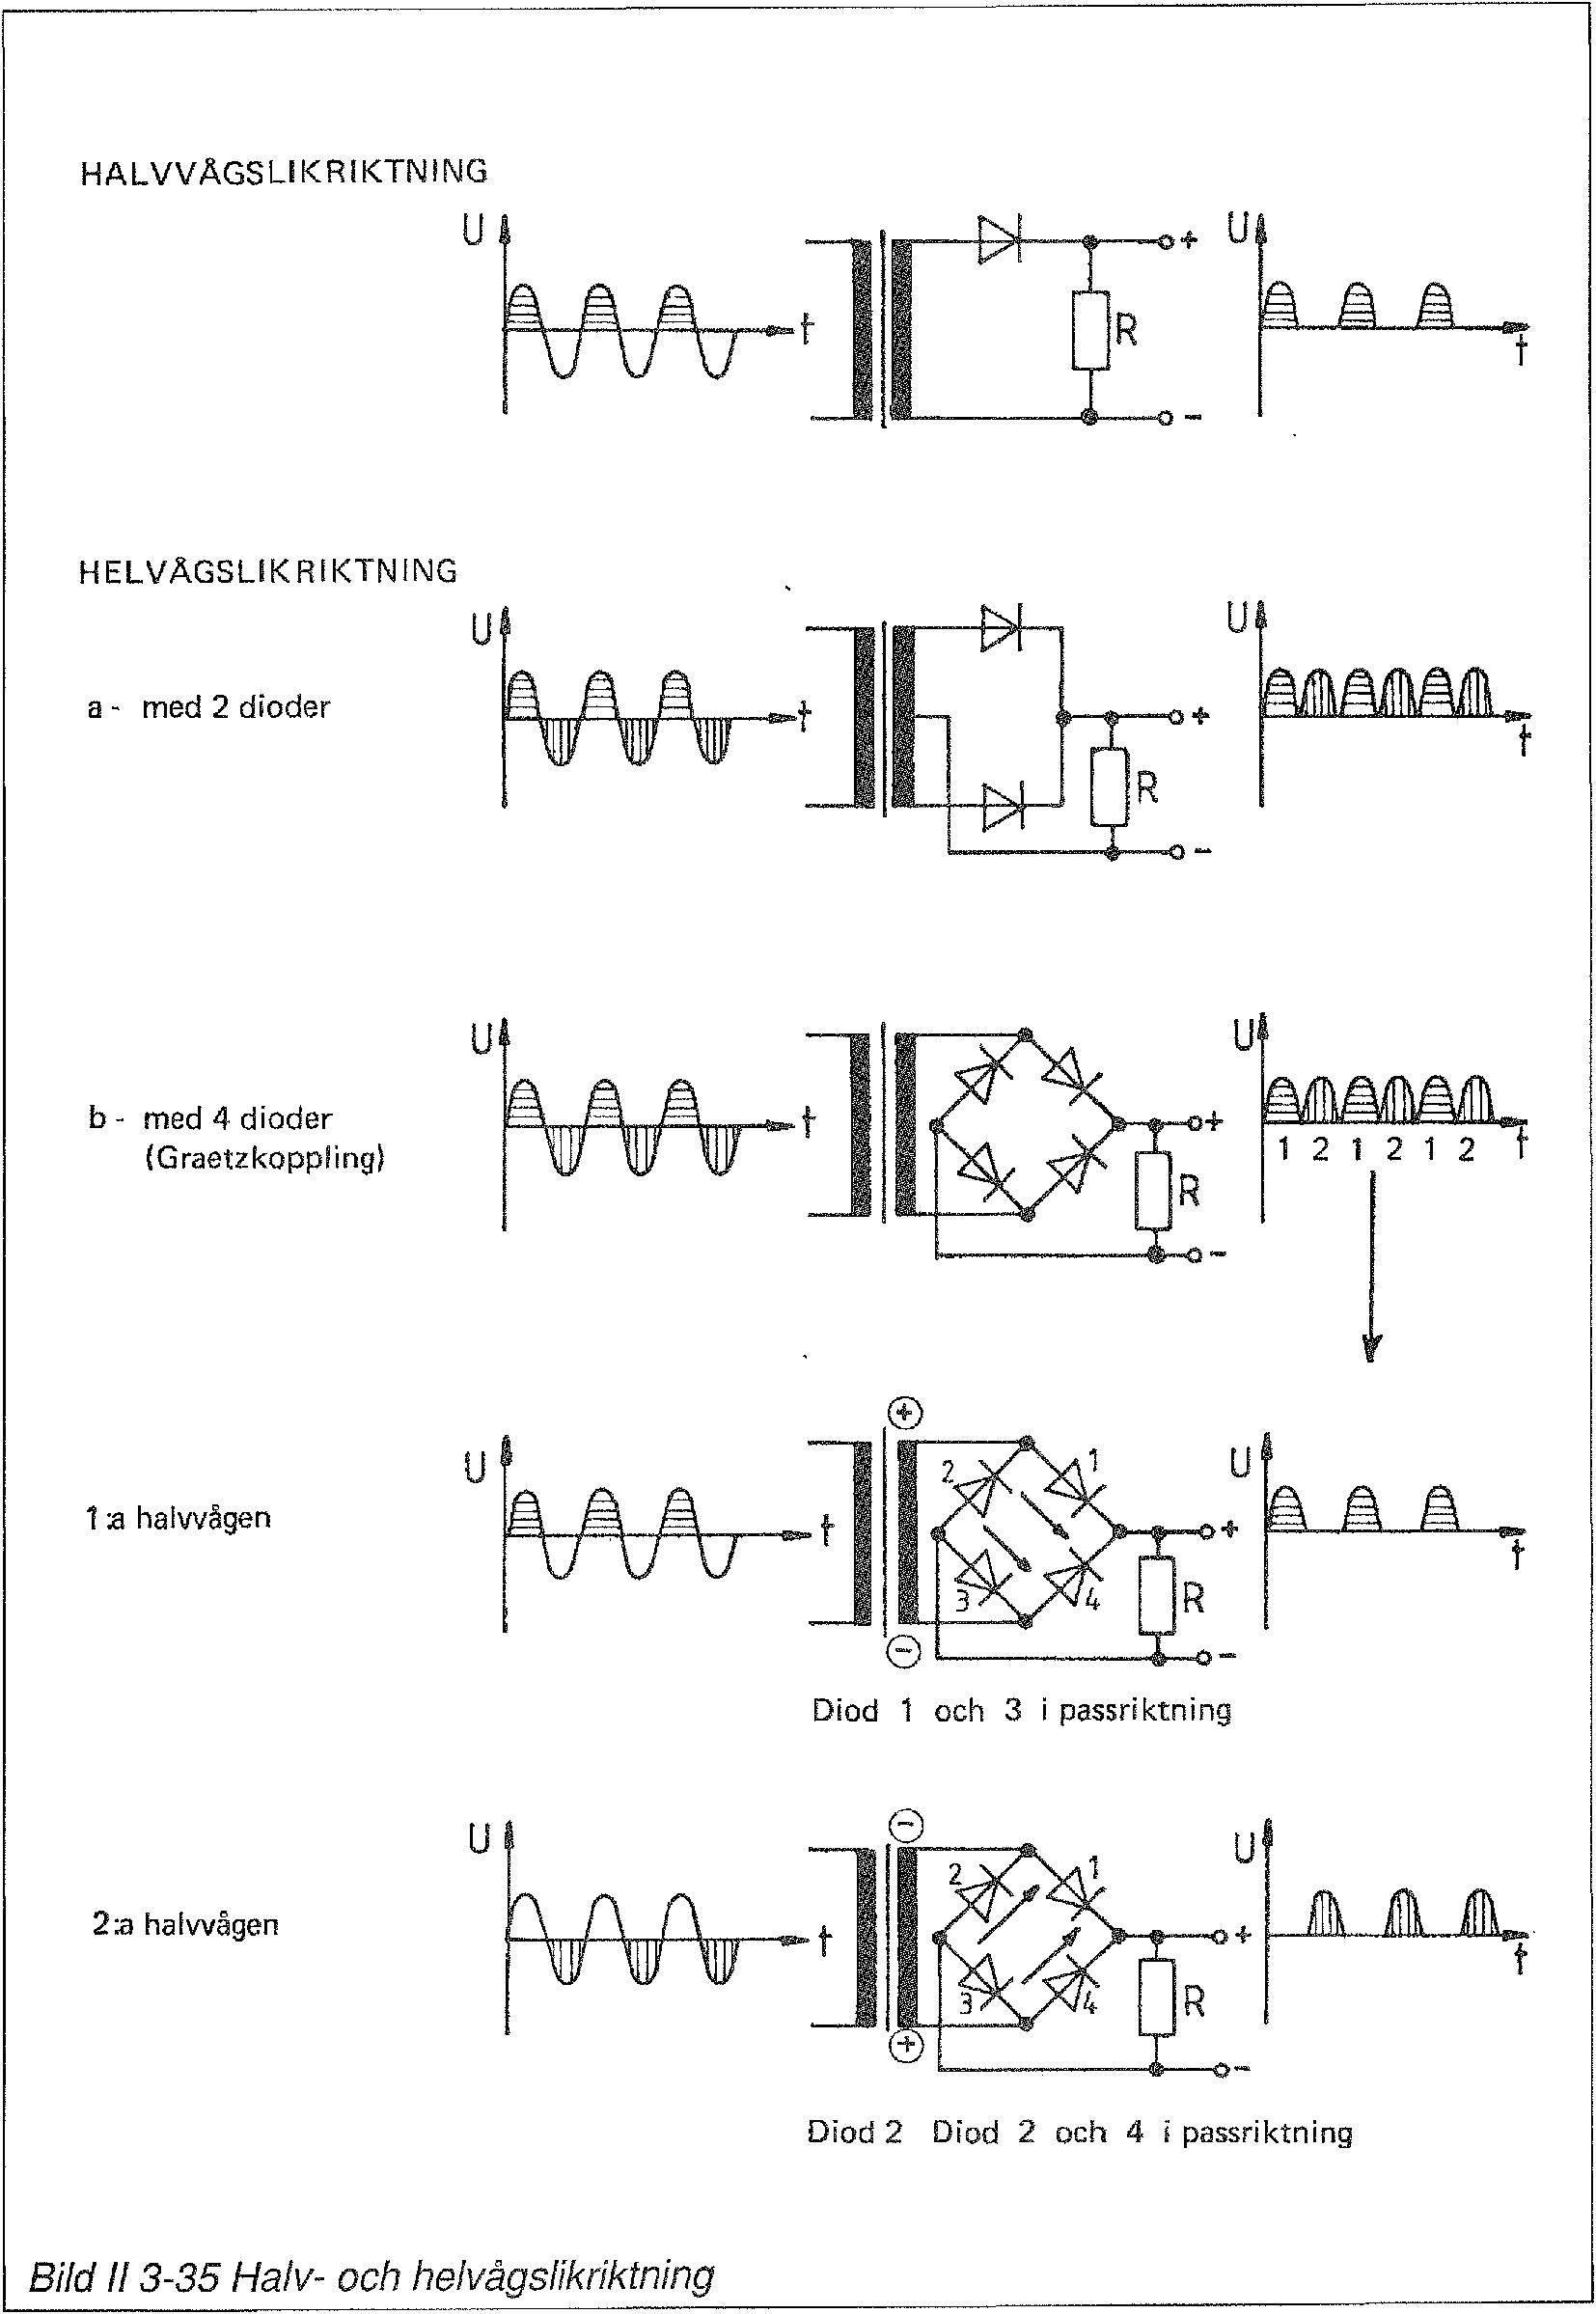
\includegraphics[width=0.8\textwidth]{images/bild_2_3-35}
%\caption{Alstring av en sinusformad signal}
\label{fig:BildII1-16}
\end{figure}
\end{frame}

\begin{frame}{Kraftaggregat -- glättning}

\begin{figure}[h]
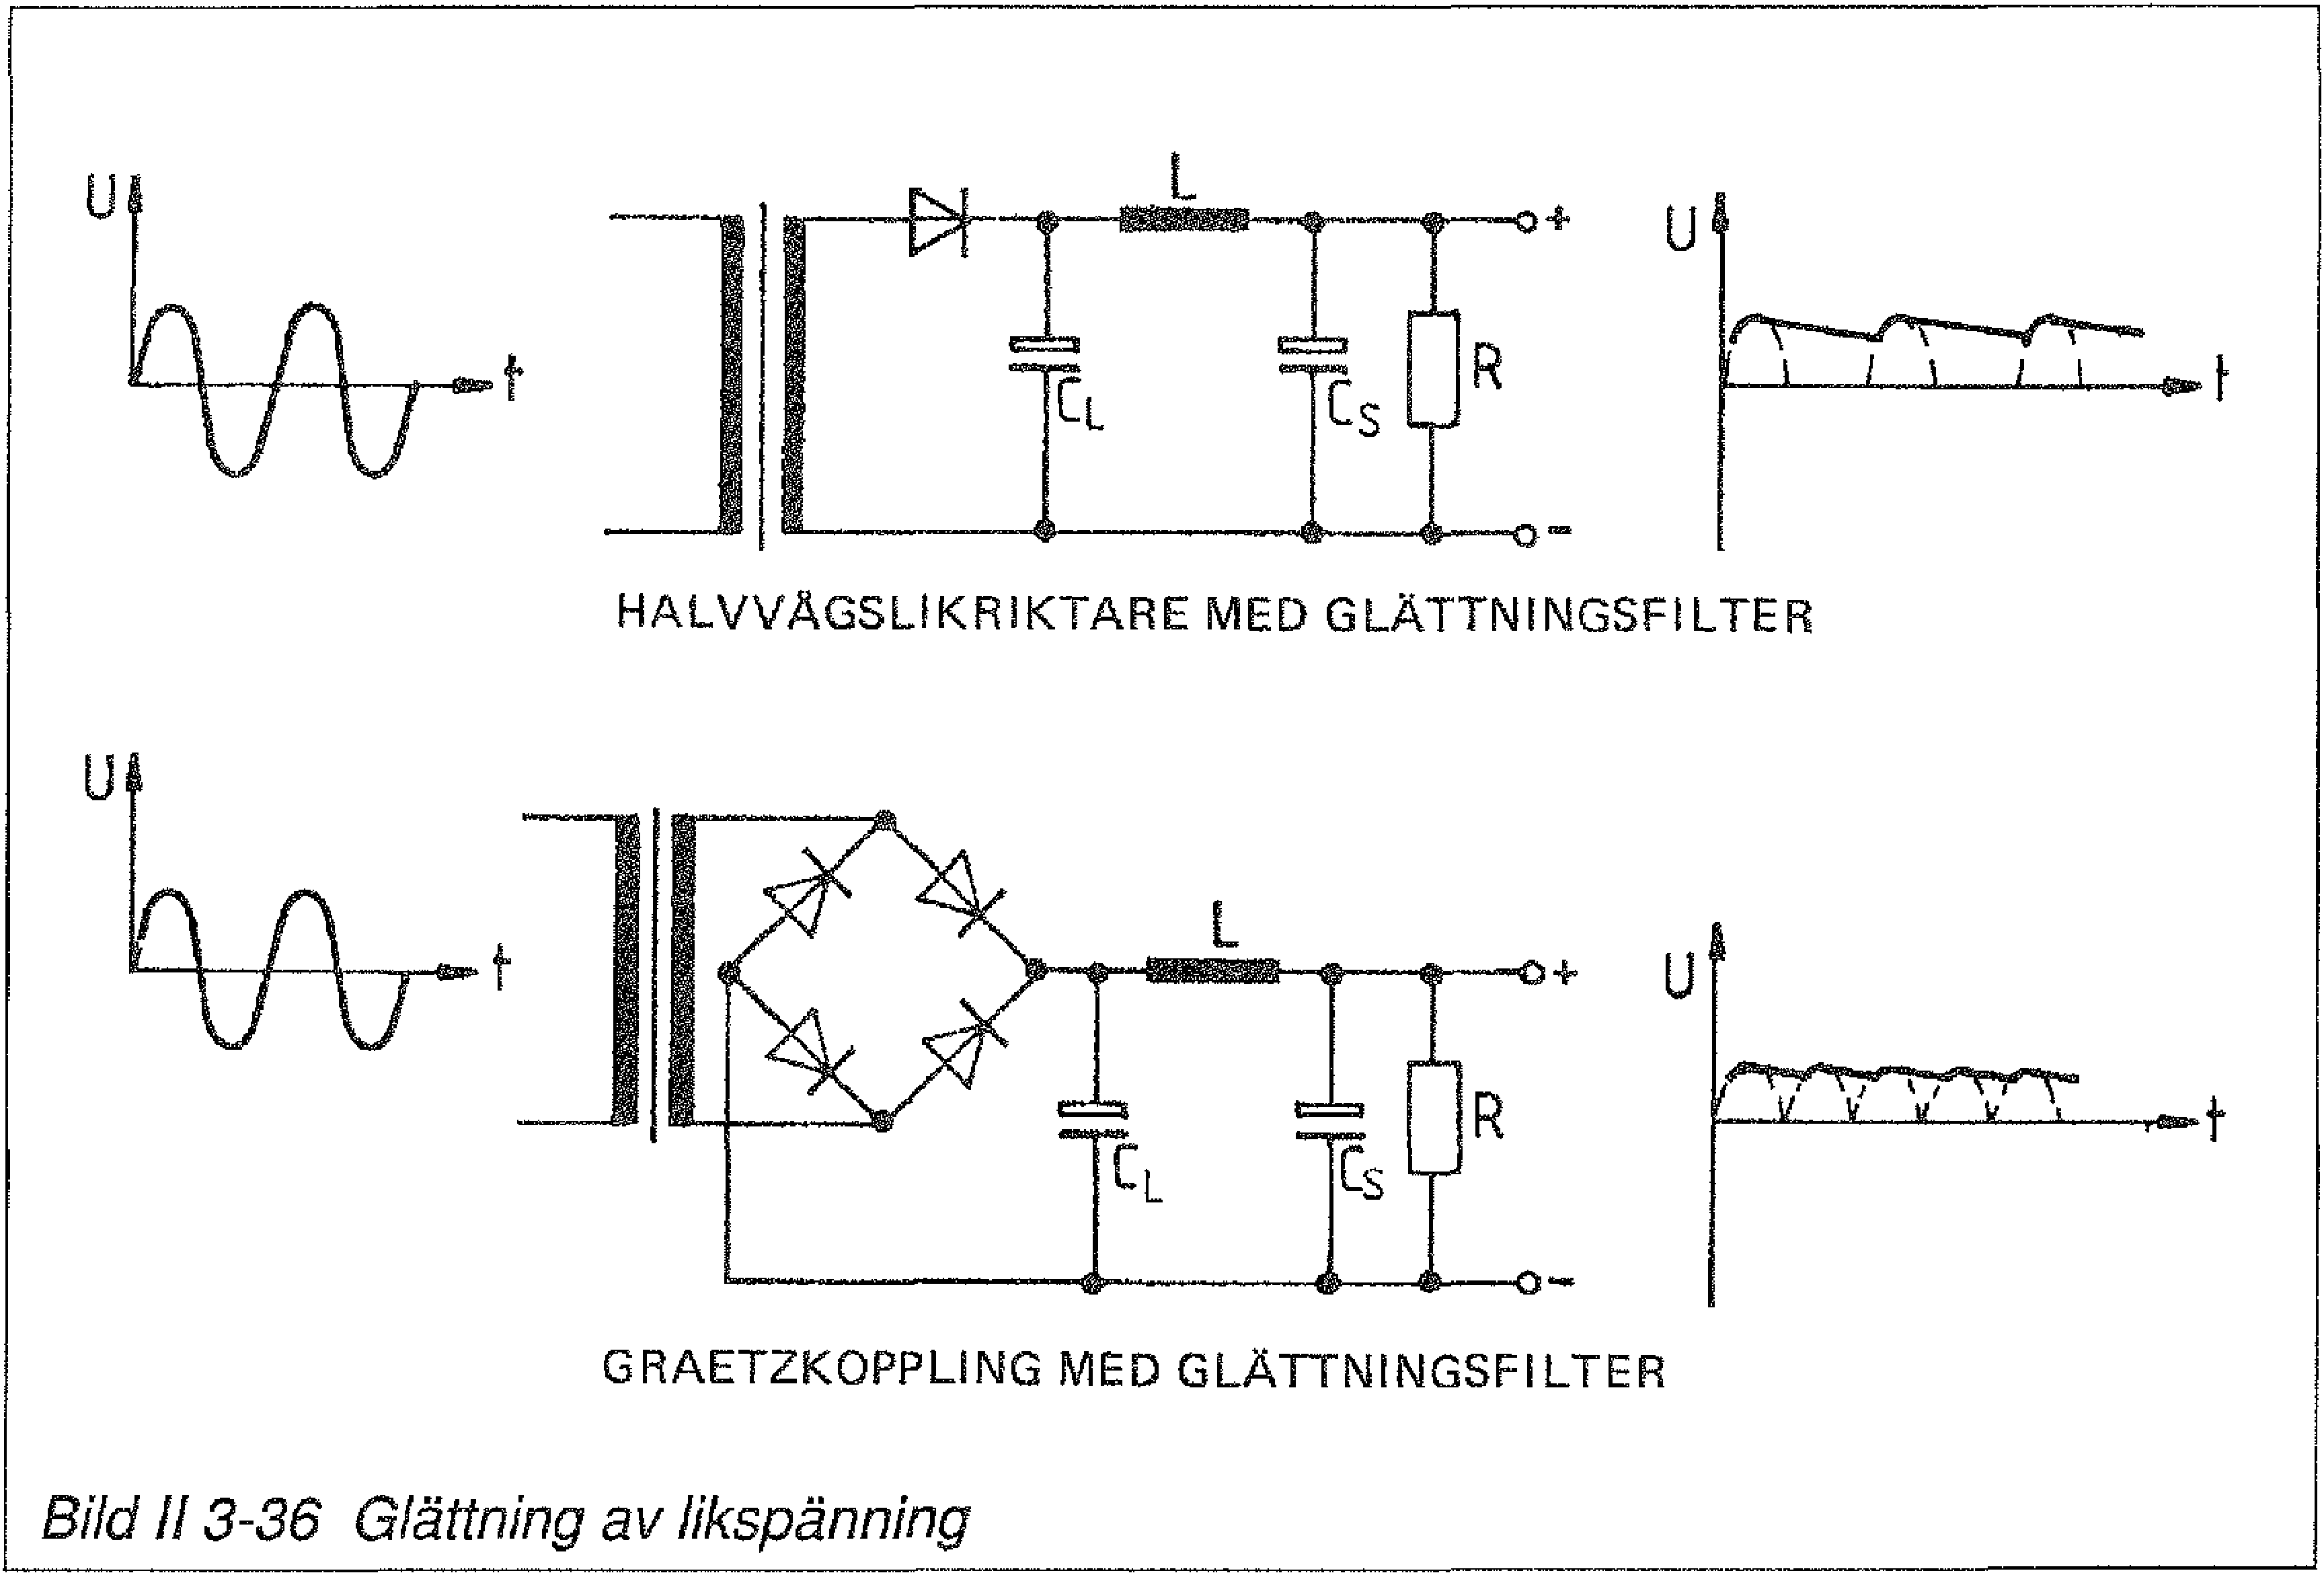
\includegraphics[width=0.8\textwidth]{images/bild_2_3-36}
%\caption{Alstring av en sinusformad signal}
\label{fig:BildII1-16}
\end{figure}
\end{frame}

\section{Transistorn}

\begin{frame}{Transistor}

\begin{figure}[h]
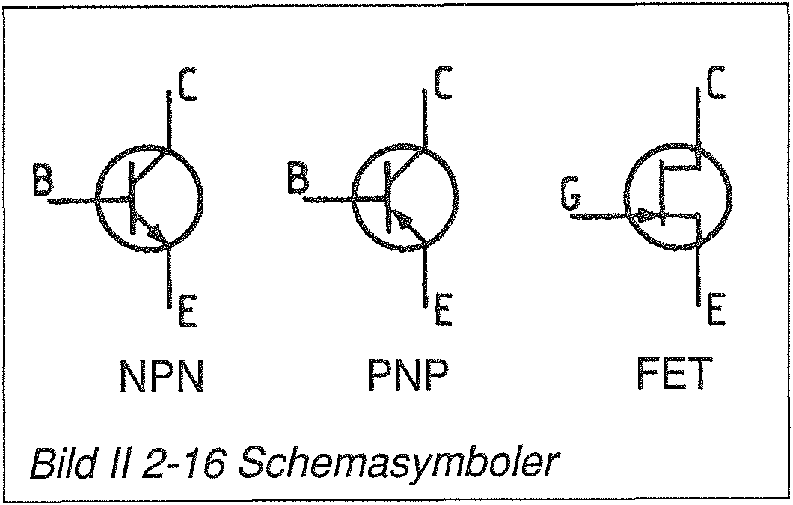
\includegraphics[width=0.4\textwidth]{images/bild_2_2-16}
\end{figure}

\begin{itemize}
  \item Dubbla PN övergångar: PNP samt NPN -- bipolära transistorer
  \item Ström-förstärkning -- en ström styr en större ström
  \item Field Effect Transistor (FET) -- elektrostatiskt fält (spänning) styr ström
\end{itemize}
\end{frame}

\begin{frame}{Strömförstärkning}

\begin{figure}[h]
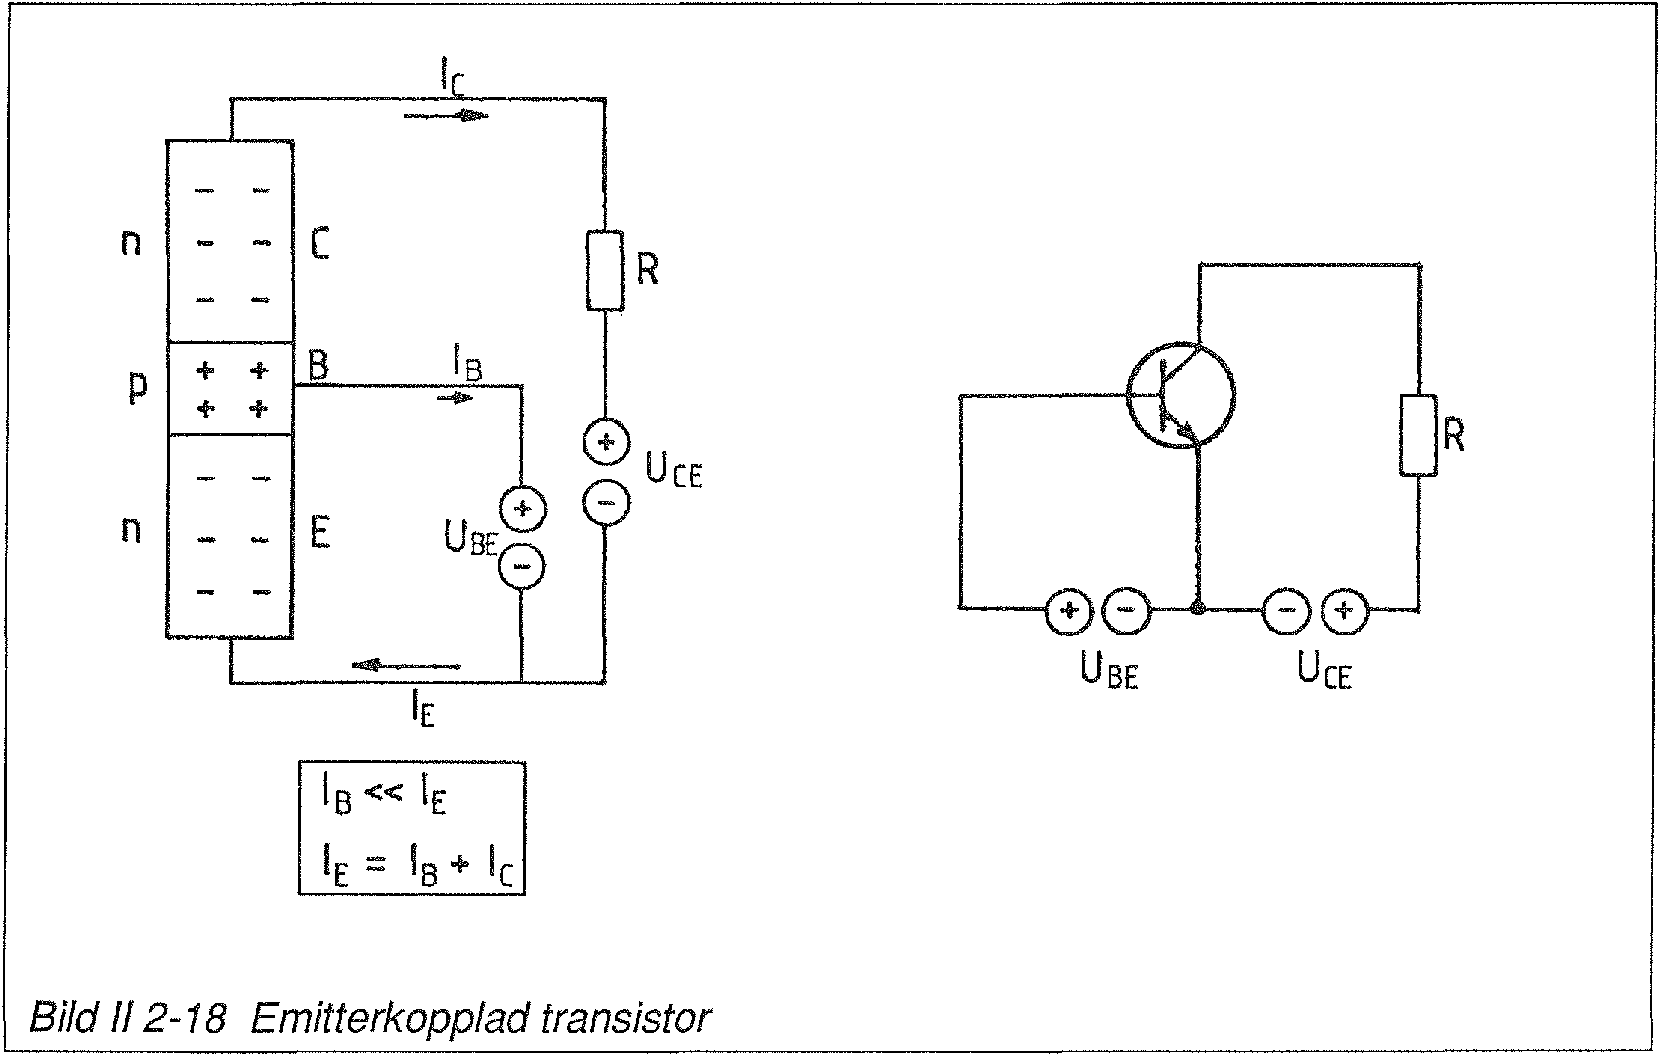
\includegraphics[width=0.6\textwidth]{images/bild_2_2-18}
\end{figure}

\begin{itemize}
    \item Strömförstärkningfaktorn $h_{FE}=\frac{\Delta I_C}{\Delta I_B}$
    \item Strömförstärkningsfaktorn $h_{FE}$ (även $\beta$) typiskt 100-600
    \item Effekt-transistorer typiskt 10-50
    \item Darlingtonpar typiskt mer än 500
  \end{itemize}
\end{frame}

\section{Förstärkare}

\begin{frame}{Förstärkare}
  \begin{itemize}
  \item Förstärkning (eng. Gain) - $G$
  \item Spänningsförstärkning - $U_{ut} = G U_{in}$
  \item Strömförstärkning - $I_{ut} = G I_{in}$
  \item Buffersteg - 1 i spänningsförstärkning -- isolerar impedanser
  \item Pre-amp/LNA -- lågbrusigt förstärkarsteg -- Low Noise Amplifier (LNA)
  \item försteg -- för-förstärkare som höjer effekten före ett PA-steg
  \item PA-steg -- Power Amplifier -- steg med hög effekt
  \end{itemize}
\end{frame}

\section{Oscillatorer}

\begin{frame}{Oscillatorer}

\begin{figure}[h]
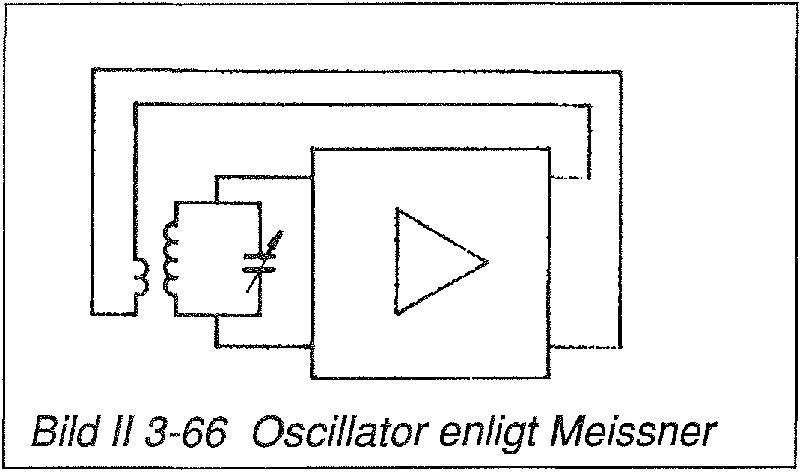
\includegraphics[width=0.4\textwidth]{images/bild_2_3-66}
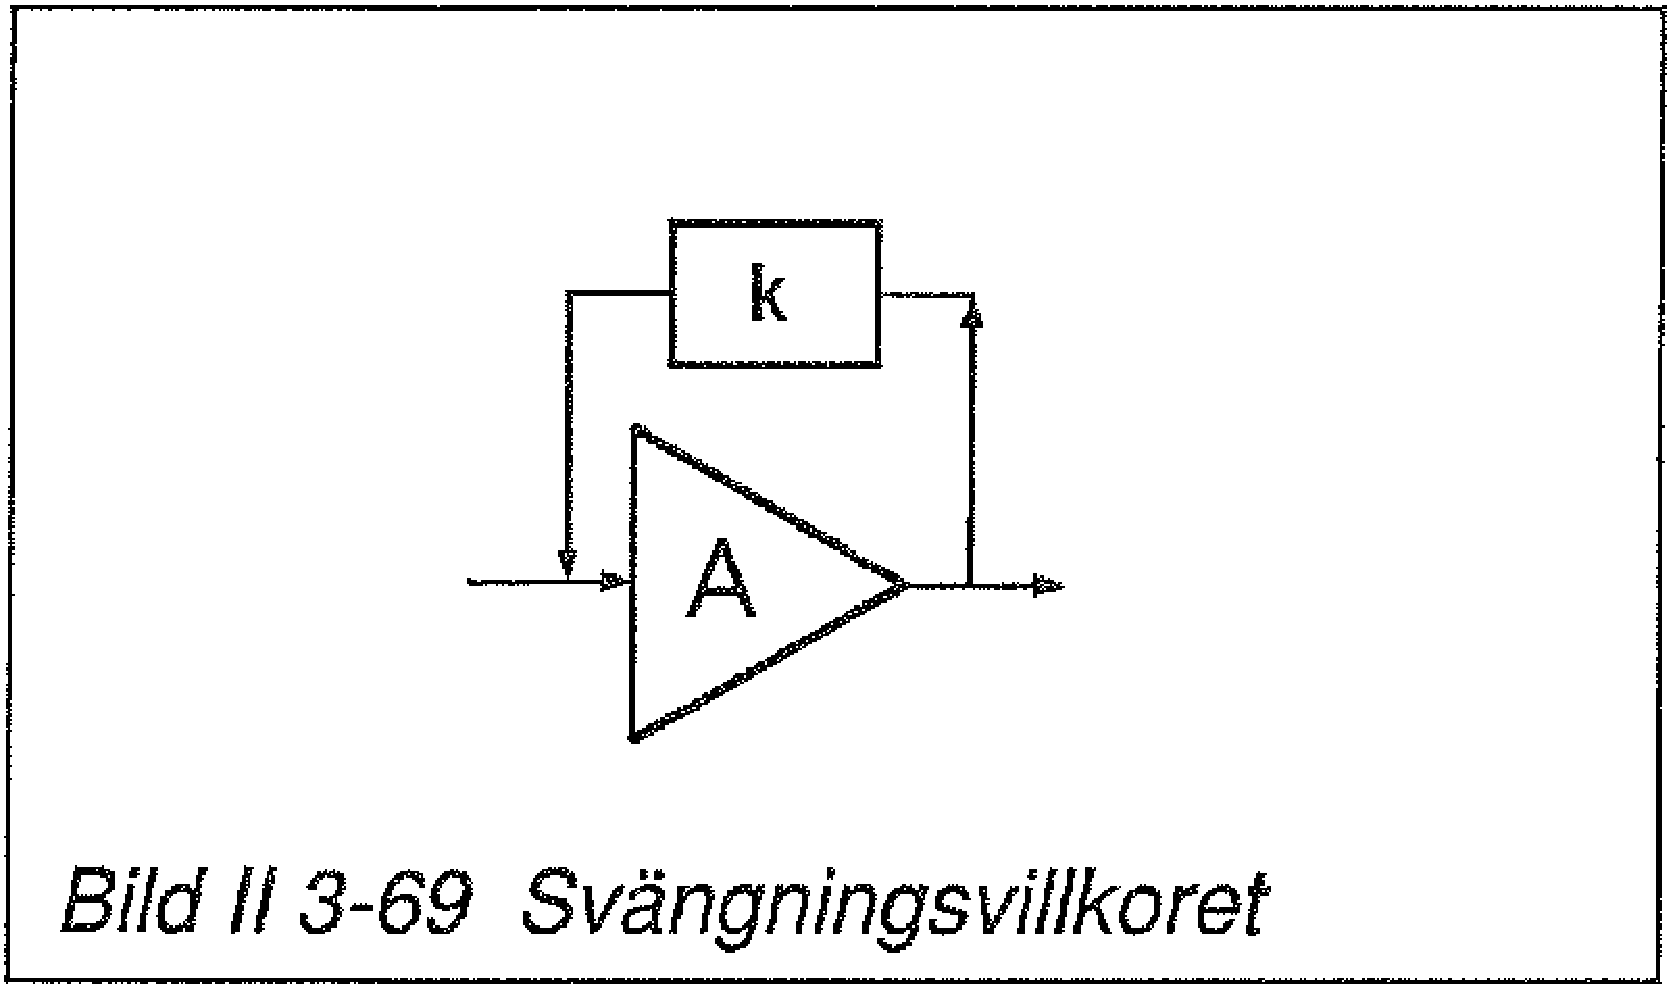
\includegraphics[width=0.4\textwidth]{images/bild_2_3-69}
\end{figure}

\begin{itemize}
\item En LC-krets har en resonanssfrekvens, men förlusten gör att amplituden
  minskar fort med tiden.
\item En förstärkare kan förstärka signalen.
\item En oscillator kombinerar resonansen med en förstärkare för att få en kontinuerlig oscillation.
\item Självsvängningsvillkoren måste vara uppfyllda: (\textbf{Överkurs!})
  \begin{itemize}
  \item Förstärkningen genom loopen vid resonansfrekvensen är 1
  \item Fasförskjutningen genom loopen vid resonansfrekvensen är 0 grader
  \end{itemize}
\end{itemize}
\end{frame}

\begin{frame}{Oscillatorer}
  \begin{itemize}
    \item Fix frekvens oscillator -- har en fix stabil frekvens, ofta en kristal-oscillator
    \item Variabel frekvens oscillator (VFO) -- har en variabel frekvens, ofta inte jättestabil
    \item Spänningsstyrd oscillator (Voltage Controlled Oscillator -- VCO) -- en spänning styr oscillatorn
    \item Temperatur-kompenserad oscillator (TCXO) -- en temperatur-sensor styr spänningen hos en VCO för att stabiliisera med avseende på temperaturvariationer
    \item Ungs-stabiliserad oscillator (OCXO) -- en temperatur-reglering håller kristallen vid en fix temperatur (ofta ca 85 grader celsius)
  \end{itemize}
\end{frame}

\section{Faslåsta loopar (PLL)}

\begin{frame}{PLL översikt}

\begin{figure}[h]
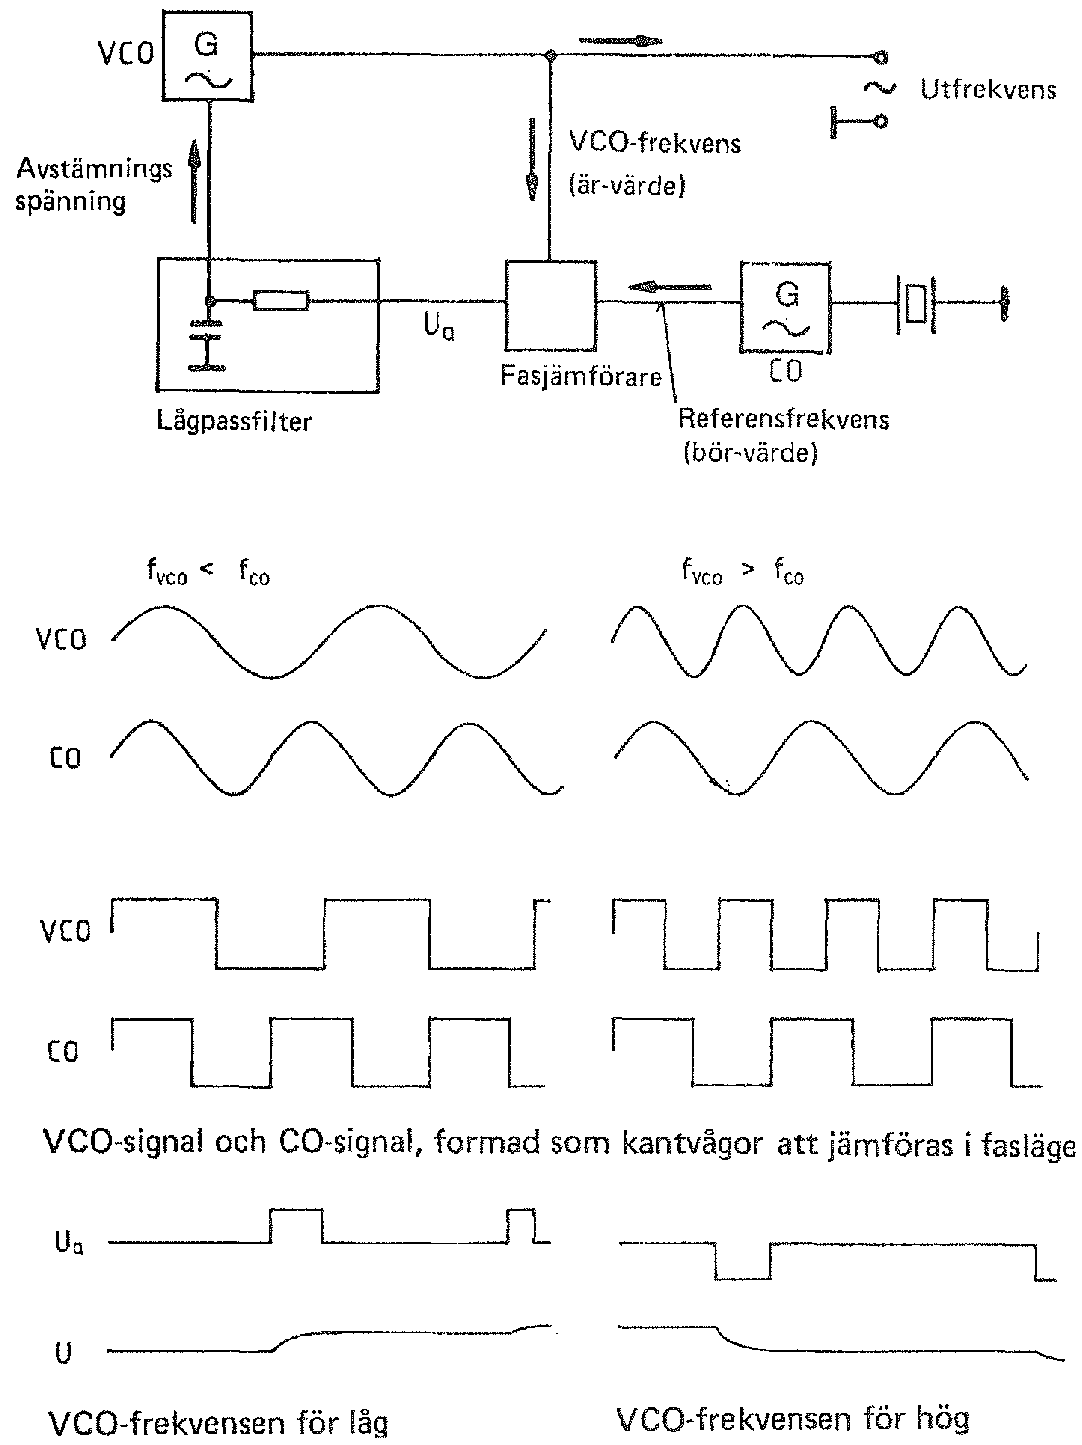
\includegraphics[width=0.5\textwidth]{images/bild_2_3-80b}
\end{figure}

\end{frame}

\begin{frame}{PLL komponenter}
  \begin{itemize}
    \item Fix oscillator -- stabil referens
    \item Spänningsstyrd oscillator -- styrd oscillator
    \item Frekvensdelare -- styrbar delning av den styrda oscillatorn
    \item Fasdetektor -- jämför fasen mellan referensoscillatorn och den (neddelade) styrda oscillatorn
    \item Lågpassfilter/loop-filter -- undertrycker störningar och skapar styrdspänning ur detekterad fas-skillnad
    \item Medger många olika frekvenser, med stabiliteten hos referensoscillatorn
  \end{itemize}
\end{frame}

\end{document}
